% COMP813 Artificial Intelligence 2026 — Final Project report
% Aung Kyaw Zay Ya (24265298), Auckland University of Technology
%
% Built on the provided cvpr2017AuthorKit template.
%
% TO STRIP EVERY DRAFTING NOTE BEFORE SUBMITTING: change \draftnotestrue
% below to \draftnotesfalse and recompile. One word, nothing else to touch.
%
% Build:  pdflatex report && pdflatex report
% (twice, so the figure and table references resolve)

\documentclass[10pt,twocolumn,letterpaper]{article}

\usepackage{cvpr}
\usepackage{times}
\usepackage{graphicx}
\usepackage{amsmath}
\usepackage{amssymb}
\usepackage{booktabs}
\usepackage{xcolor}
\usepackage[breaklinks=true,bookmarks=false]{hyperref}

\cvprfinalcopy

\def\cvprPaperID{24265298}
\def\httilde{\mbox{\tt\raisebox{-.5ex}{\symbol{126}}}}
\ifcvprfinal\pagestyle{empty}\fi

% Drafting notes. Flip this one word to turn them all off for submission.
\newif\ifdraftnotes
\draftnotestrue          % <<< \draftnotesfalse for the submitted PDF

\newcommand{\TODO}[1]{\ifdraftnotes
  \par\noindent\fcolorbox{orange!60}{yellow!12}{%
    \parbox{0.95\linewidth}{\footnotesize\textbf{TODO}\ \textit{#1}}}\par\medskip
\fi}

% APA 7 reference list: alphabetical, hanging indent, no numbering.
\newenvironment{apareferences}%
  {\section*{References}\small
   \setlength{\parindent}{-0.22in}\setlength{\leftskip}{0.22in}%
   \setlength{\parskip}{5pt}}%
  {\par}

\begin{document}

\title{No Model Wins Everything: A Multi-Objective Evaluation of a\\
       Nested Hybrid Movie Recommender}

\author{Aung Kyaw Zay Ya \quad (AUT ID 24265298)\\
School of Engineering, Computer and Mathematical Sciences\\
Auckland University of Technology\\
{\tt\small <your AUT student email>}}

\maketitle

\TODO{Replace the email placeholder in the author block with your AUT student address, and confirm the title.}

%%%%%%%%%%%%%%%%%%%%%%%%%%%%%%%%%%%%%%%%%%%%%%%%%%%%%%%%%%%%%%%%%%%%%%%%%%%
\begin{abstract}
Recommender systems are usually reported with a single headline number, and
the choice of that number decides which system looks best. This project builds
seven movie recommenders on MovieLens \texttt{ml-latest-small} and evaluates
all of them on one held-out split under five families of measure: rating
error, ranking quality, catalogue coverage, beyond-accuracy quality (novelty
and serendipity), and cold-start reach. The models are a damped-bias SVD, an
item-based autoencoder (I-AutoRec), a TF-IDF content model over TMDB plot
overviews, three hybrid compositions of those, and a non-personalized
Most-Popular baseline. The central result is that no model wins everything:
across six measures, three different models hold the six titles. I-AutoRec
attains the lowest rating error (RMSE 0.8517) while recommending from 0.6\% of
the catalogue, a figure identical to the non-personalized baseline's, and its
novelty of 1.86 sits nearer that baseline's 1.65 than the 7.13 a uniformly
random recommender would score. The content model is the most diverse (24.9\%
coverage, novelty 6.76, 481 cold-start slots) and the worst ranker (NDCG@10
0.0359). A nested hybrid, a recommender whose first component is itself a
hybrid, ranks best (NDCG@10 0.1643). Because a single split cannot separate
small differences, the entire comparison is repeated across four splits: eight
of ten reported claims hold on every split, while the claim that SVD fails to
beat the popularity baseline does not. That paired difference is $+0.0012$
NDCG@10 and changes sign twice, so collaborative filtering alone is better
described as indistinguishable from recommending best-sellers than as worse
than it. The weighted hybrids, by contrast, beat plain SVD on every split by
$+0.0103 \pm 0.0022$.
\end{abstract}

%%%%%%%%%%%%%%%%%%%%%%%%%%%%%%%%%%%%%%%%%%%%%%%%%%%%%%%%%%%%%%%%%%%%%%%%%%%
\section{Introduction}

A catalogue of ten thousand films is larger than any viewer can inspect, so
the practical question is not whether to filter it but how. Recommender
systems answer that by estimating preference from past interactions and
ranking the catalogue accordingly. The research literature has converged on a
small set of measures for judging how well they do it --- rating error for
predicted scores, and precision, recall and normalized discounted cumulative
gain for ranked lists --- and a system is normally reported by one of them.

That convention hides something. A model can score well on rating error by
predicting confidently on the films almost everyone has already rated, and a
ranking metric can only credit a recommendation whose item somebody in the
test set happened to rate. Both measures therefore reward concentration on
popular items, and neither penalises a system that never recommends anything
else. Whether that matters is an empirical question, and it is the question
this project asks.

\noindent\textbf{Research question.} \textit{Can a hybrid recommender improve
on its individual components, and does ``improve'' mean the same thing when
quality is measured by accuracy, by catalogue behaviour, and by novelty?}

\noindent Four objectives follow from it:

\begin{enumerate}\itemsep2pt
\item Implement and evaluate three recommenders of different families
      (matrix factorization, deep autoencoder, content-based NLP) on a
      common split.
\item Compose them into hybrids by weighted blending, switching and nesting,
      rather than treating a three-model blend as a new algorithm.
\item Measure all seven systems on the same held-out data under rating error,
      ranking, coverage, novelty, serendipity and cold-start reach.
\item Quantify how far the resulting conclusions depend on the particular
      train/test split they were measured on.
\end{enumerate}

\noindent The contributions are:

\begin{itemize}\itemsep2pt
\item A composable hybrid in which a hybrid is itself a valid component, so a
      three-model system is a two-line composition rather than a rewrite
      (Section~\ref{sec:hybrid}).
\item A seven-model comparison under five metric families, showing that three
      different models hold the six available titles
      (Section~\ref{sec:beyond}).
\item Evidence that the deep model's advantage in rating error is bought by
      collapsing onto popular items: its catalogue coverage equals the
      non-personalized baseline's to one decimal place, and its novelty is
      closer to that baseline than to chance.
\item A proof that cold-start failure here is a property of the data rather
      than of model capacity: for items with no training ratings, both the
      linear and the non-linear model produce predictions with exactly zero
      variance (Section~\ref{sec:cold}).
\item A robustness check that repeats the whole comparison on four splits and
      identifies which reported claims survive (Section~\ref{sec:robust}).
\end{itemize}

%%%%%%%%%%%%%%%%%%%%%%%%%%%%%%%%%%%%%%%%%%%%%%%%%%%%%%%%%%%%%%%%%%%%%%%%%%%
\section{Related Work}

\subsection{Collaborative filtering and matrix factorization}
Collaborative filtering estimates preference from the user--item interaction
matrix alone. Sarwar et al. (2001) moved the neighbourhood computation from
users to items, arguing that item--item relationships are more stable and can
be precomputed. Matrix factorization replaced explicit neighbourhoods with
latent factors; Koren et al. (2009) set out the formulation used here,
including the user and item bias terms that account for the systematic
tendency of some raters to rate high and some films to be rated high. This
project uses a truncated singular value decomposition of the mean-centred
matrix with a damped item-bias term, which is the same idea in its simplest
form.

\subsection{Deep collaborative filtering}
Autoencoder and neural formulations aim to capture interaction patterns that
an inner product cannot. Sedhain et al. (2015) proposed AutoRec, an
autoencoder that reconstructs a partially observed rating vector under a loss
masked to the observed entries; the item-based variant, I-AutoRec, treats each
item's vector of user ratings as one training example and is the variant
implemented here. He et al. (2017) generalised the idea, replacing the inner
product with a learned interaction function. Both report accuracy gains over
matrix factorization. Neither is evaluated on catalogue behaviour, which is
the gap this project addresses for I-AutoRec specifically.

\subsection{Content-based and hybrid recommendation}
Content-based methods score items by similarity to what the user has already
liked, using item descriptions rather than co-rating patterns, and so remain
defined for items with no interaction history at all. Burke (2002) provides
the taxonomy this project follows directly: the weighted hybrid combines
component scores numerically, while the switching hybrid selects a component
per case according to a criterion. The nesting used in
Section~\ref{sec:hybrid} is a composition of weighted hybrids rather than a
new category in that taxonomy.

\subsection{Beyond-accuracy objectives}
Kaminskas and Bridge (2016) survey the measures used when recommendation
quality is treated as more than predictive accuracy, and give the definitions
of novelty and serendipity adopted in Section~\ref{sec:metrics}: novelty as
the self-information of a recommended item, and serendipity as relevance
discounted by how expected the item was. Adomavicius and Kwon (2012) show
that aggregate diversity can be improved substantially at a small accuracy
cost, which is the trade-off this project measures rather than assumes.

\subsection{Evaluation methodology}
Cremonesi et al. (2010) report that on top-$N$ tasks a non-personalized
popularity baseline is far stronger than its reputation, and that models tuned
for rating error do not necessarily rank well. Both observations recur in
Section~\ref{sec:ranking}. Meng et al. (2020) show that the choice of data
splitting strategy materially changes which model appears best, which
motivates the robustness check in Section~\ref{sec:robust}. Panda and Ray
(2022) review cold-start mitigation and note that the right strategy depends
on whether the cold entity is a user or an item and on what side information
exists --- a distinction Section~\ref{sec:cold} relies on.

\TODO{Verify every reference against the original paper or its DOI before
submitting. Related Work is worth 10\% of the report mark; adding one or two
references you find yourself is worth the time.}

%%%%%%%%%%%%%%%%%%%%%%%%%%%%%%%%%%%%%%%%%%%%%%%%%%%%%%%%%%%%%%%%%%%%%%%%%%%
\section{Data}

\subsection{MovieLens \texttt{ml-latest-small}}
All experiments use the MovieLens \texttt{ml-latest-small} benchmark
(Harper \& Konstan, 2015): 100,836 ratings on a half-star scale from 0.5 to
5.0, contributed by 610 users across 9,724 distinct rated films. The full
catalogue file lists 9,742 titles; the 18 with no ratings never enter the
user--item matrix. That matrix is therefore $610 \times 9{,}724$ with 98.3\%
of its cells empty. Every user in the release has rated at least 20 films, so
there are no cold \emph{users} here --- the cold-start problem measurable in
this dataset is entirely item-side.

\subsection{TMDB plot overviews}
The content model needs text. Plot overviews were fetched from The Movie
Database using the \texttt{tmdbId} column of the benchmark's
\texttt{links.csv}, giving 9,603 of the 9,724 rated films (98.8\%). The 121
that remain uncovered are not a collection gap: 113 have no synopsis on TMDB
at all and 8 carry no \texttt{tmdbId}, so they are not fetchable.
Appendix~\ref{app:tmdb} reports what expanding this coverage did to the
content model, which is not what was expected.

\subsection{Split protocol}
Each user's ratings are shuffled and split 60/20/20 into train, validation and
test. Splitting per user rather than globally guarantees every user appears in
all three parts, so no user is unmeasurable at evaluation time. The shuffle is
seeded with the author's student ID, and the test slice is taken before the
validation slice is carved out, so a two-way and a three-way split of the same
seed select identical test rows. Hyperparameters are selected on validation
only; models are then refitted on train${+}$validation and the test set is
evaluated exactly once per model.

\subsection{Cold items}
732 of the 9,724 films receive no rating at all in the combined
train${+}$validation portion, and 794 test ratings fall on them. These are the
\emph{cold items} referred to throughout. They are 7.5\% of the catalogue but
only 2.92\% of the relevant held-out ratings, and that asymmetry explains much
of Section~\ref{sec:cold}.

%%%%%%%%%%%%%%%%%%%%%%%%%%%%%%%%%%%%%%%%%%%%%%%%%%%%%%%%%%%%%%%%%%%%%%%%%%%
\begin{figure*}[t]
\centering
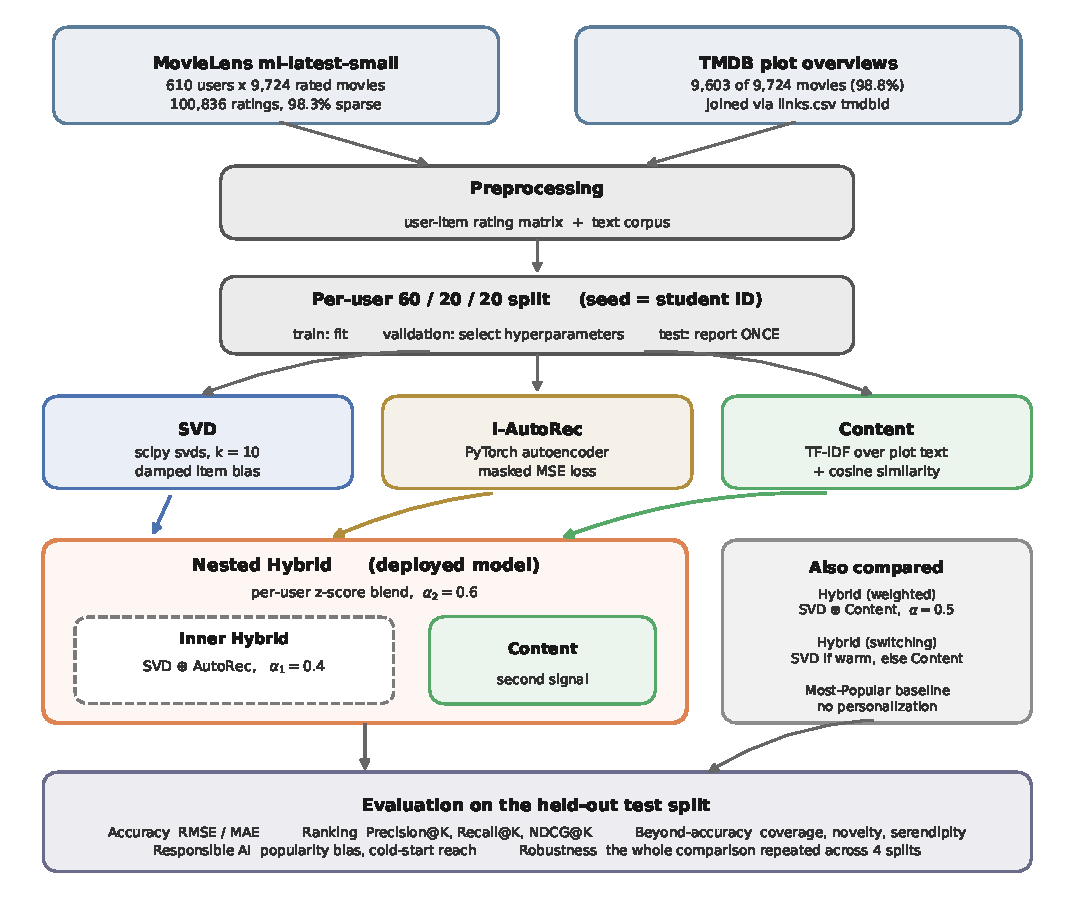
\includegraphics[width=0.98\textwidth]{fig1_architecture.pdf}
\caption{Model architecture. Data, the three-way split, the three base models,
the nested composition, the ablation variants and the evaluation battery. The
nested hybrid is drawn as a box inside a box because that is what it is: a
hybrid whose first component is another hybrid, not a special-cased three-way
blend.}
\label{fig:arch}
\end{figure*}

\section{Methods}

\subsection{Matrix factorization (SVD)}
The rating matrix is mean-centred, missing entries are filled with zero, and a
truncated SVD retains the $k$ largest singular values. Reconstruction adds the
centring back and clips to the valid rating range. An item-bias term is added,
damped as the sum of an item's residuals divided by its rating count plus a
damping constant, so an item with two ratings is shrunk toward zero bias while
one with two hundred is not. Two centring modes are used: subtracting the user
mean only, and subtracting the user mean and then the item bias. The
validation grid selected $k=10$ with damping $=5$.

The behaviour on cold items follows from the construction and is worth stating
because Section~\ref{sec:cold} tests it. An item with no training ratings
contributes an all-zero column to the centred matrix, so the reconstruction
contributes nothing and the predicted rating is exactly the user's own mean,
for every such item.

\subsection{I-AutoRec}
The item-based autoencoder (Sedhain et al., 2015) takes each item's
610-dimensional vector of user ratings as one training example, encodes it
through a sigmoid layer of width $h$, and decodes it linearly. The loss is
mean squared error masked to the observed entries, so unobserved cells
contribute no gradient. Training uses Adam with weight decay as the
regularizer and early stopping on validation error. Two configurations are
carried forward because the validation grid selected different ones for the
two metric families --- $h=200$ with weight decay $10^{-4}$ minimised
validation RMSE, while $h=25$ with weight decay $10^{-2}$ maximised validation
NDCG@10 --- and reporting one model under both headings would misrepresent it.
Appendix~\ref{app:grids} gives the grid.

The same cold-item argument applies here and is sharper. A cold item's input
vector is entirely zero, so the encoder sees the same input for every cold
item and the decoder can only emit its own bias. Every cold item therefore
receives an identical prediction, for a given user, regardless of which film
it is. Non-linearity does not help, because there is no signal for the
non-linearity to act on.

\subsection{Content-based model}
Plot overviews are vectorised with TF-IDF and items compared by cosine
similarity. A user profile is the similarity-weighted average of the items
they rated, centred on the user's mean rating so a below-average rating pushes
away from an item rather than weakly toward it. The model scores only items
that have text, which is 98.8\% of the catalogue but never all of it, and
unlike the collaborative models it is defined for an item that has never been
rated. Genre tokens were tested as an additional feature and rejected on
validation (Section~\ref{sec:ablation}).

Because the model outputs a centred similarity rather than a rating on the
0.5--5 scale, a rating error against it is undefined, not merely unmeasured.
The implementation refuses to compute one rather than returning a misleading
figure.

\subsection{Hybrid composition}\label{sec:hybrid}
Component scores are not comparable in raw form: an SVD reconstruction lives
on the rating scale and a content score is a centred cosine similarity. Each
component's scores are therefore standardised per user to zero mean and unit
variance before combining, so the blend weight controls the relative influence
of the two signals rather than the relative size of their units.

Two of Burke's (2002) strategies are implemented. The weighted hybrid returns
$\alpha\,z_1 + (1-\alpha)\,z_2$ over the standardised component scores. The
switching hybrid uses the first component where it has a collaborative signal
and the second where it does not, which is what makes it the variant with the
most cold-start reach in Section~\ref{sec:cold}.

The design decision that matters is that a hybrid accepts any component
satisfying the same small interface, and a hybrid satisfies that interface
itself. A three-model system is therefore a composition of two two-model
hybrids rather than a separate implementation:
\begin{center}
\texttt{Hybrid( Hybrid(SVD, AutoRec, $\alpha_1$), Content, $\alpha_2$ )}
\end{center}
The consequence is not only brevity. Because the components stay separate
objects, each can still be measured on its own, which is what makes the
attribution in Section~\ref{sec:beyond} possible. A single model trained
end-to-end on all three signals would rank better or worse as one number, with
no way to say which signal produced the difference.

\subsection{Baselines}
Three baselines are used. The user-mean predictor bounds the rating-error
results from below in difficulty. An off-the-shelf scikit-learn
\texttt{TruncatedSVD} without the item-bias term isolates the contribution of
that term. Most-Popular, which ranks every user's unseen items by training-set
rating count, is the ranking baseline; following Cremonesi et al. (2010) it is
treated as a serious competitor rather than a formality, and
Section~\ref{sec:ranking} shows why.

\subsection{Evaluation measures}\label{sec:metrics}
Five families are reported.

\begin{itemize}\itemsep2pt
\item \textbf{Rating error.} RMSE and MAE over test ratings the model can
      score. Only the SVD and AutoRec produce calibrated ratings, so this
      applies to two of the seven systems.
\item \textbf{Ranking.} Precision@$K$, Recall@$K$ and NDCG@$K$ at
      $K \in \{5,10,20\}$, with an item counted relevant if rated $\geq 4.0$
      in the test split. Precision divides by $K$ rather than by the returned
      list length, so a model returning a short list is charged for the
      unfilled slots instead of flattered by them.
\item \textbf{Catalogue coverage.} The fraction of the catalogue appearing in
      at least one user's top-10, reported against the whole catalogue and
      against each model's reachable pool.
\item \textbf{Novelty and serendipity.} Novelty is the mean self-information
      $-\log_2 p(i)$ of recommended items, with add-one smoothing so the 732
      unrated items score the highest finite value rather than infinity.
      Serendipity is Precision@10 with each hit weighted by $1-p(i)$; it
      shares Precision's denominator and $0$--$1$ scale, so the ratio of the
      two reads as the share of a model's accuracy that came from something
      other than best-sellers.
\item \textbf{Cold-start reach.} The number of top-10 slots, out of 6,100,
      occupied by items with no train${+}$validation ratings.
\end{itemize}

Novelty needs a scale to be read against, and two reference points are
reported with it: a uniformly random recommender scores the catalogue average
of 7.13, and an item nobody has rated scores the ceiling of 9.26. The single
most-rated film scores 1.19.

%%%%%%%%%%%%%%%%%%%%%%%%%%%%%%%%%%%%%%%%%%%%%%%%%%%%%%%%%%%%%%%%%%%%%%%%%%%
\section{Experiments}

\subsection{Setup}
All randomness is seeded with the student ID, so the split and every reported
figure reproduce exactly. Hyperparameters are selected on validation, models
are refitted on train${+}$validation, and the test split is evaluated once.

\subsection{Hyperparameter selection}
The SVD was searched over $k \in \{5,10,15,20,30,50\}$ crossed with damping
$\in \{1,5,10,25,50\}$. The content model was tested with and without genre
tokens. The blend weight $\alpha$ was swept from 0.0 to 1.0 in steps of 0.1
under two fallback strategies. I-AutoRec was searched over hidden width
$\in \{25,200\}$ crossed with weight decay
$\in \{10^{-5},10^{-4},10^{-3},10^{-2}\}$. The nested hybrid's two alphas were
searched jointly. Appendix~\ref{app:grids} reports the grids.

\subsection{Rating error}
\begin{table}[t]\centering\small
\begin{tabular}{lccc}
\toprule
Model & MSE & RMSE & MAE \\
\midrule
User-mean baseline              & 0.8927 & 0.9448 & 0.7353 \\
sklearn TruncatedSVD ($k{=}10$) & ---    & 0.9153 & 0.7063 \\
SVD ($k{=}10$, damp${=}5$)      & 0.7628 & 0.8734 & 0.6663 \\
I-AutoRec ($h{=}200$)           & \textbf{0.7253} & \textbf{0.8517} & \textbf{0.6562} \\
\bottomrule
\end{tabular}
\caption{Test rating error. The test split is touched once.}
\label{tab:rmse}
\end{table}

Table~\ref{tab:rmse} shows two things. The damped item-bias term is worth
0.0419 RMSE against an otherwise comparable library implementation without it,
a larger gain than the difference between several of the models compared
later. And the deep model beats the linear one by 0.0217 RMSE. On this
evidence alone I-AutoRec is the best model in the project, which is precisely
the conclusion the rest of this section undermines.

\subsection{Ranking}\label{sec:ranking}
\begin{table}[t]\centering\small
\begin{tabular}{lccc}
\toprule
Model & @5 & @10 & @20 \\
\midrule
SVD                       & 0.1596 & 0.1502 & 0.1456 \\
Content                   & 0.0401 & 0.0359 & 0.0345 \\
Hybrid (weighted)         & 0.1731 & 0.1605 & 0.1568 \\
Hybrid (switching)        & 0.1560 & 0.1474 & 0.1430 \\
Most-Popular              & 0.1641 & 0.1549 & 0.1562 \\
I-AutoRec                 & 0.1562 & 0.1432 & 0.1382 \\
Nested Hybrid             & \textbf{0.1796} & \textbf{0.1643} & \textbf{0.1610} \\
\bottomrule
\end{tabular}
\caption{NDCG@$K$ on the test split. Plain SVD does not beat the
non-personalized baseline at any of the three cutoffs.}
\label{tab:ndcg}
\end{table}

Plain SVD loses to Most-Popular at all three cutoffs, and I-AutoRec loses to
it more heavily. This reproduces the effect Cremonesi et al. (2010) report: a
model selected for rating error is not thereby a good ranker, and a popularity
baseline is a harder target than it looks. Only the weighted hybrids clear it.
Section~\ref{sec:robust} revisits the SVD comparison, because the margin is
small enough to be worth testing.

\subsection{Beyond accuracy: the central result}\label{sec:beyond}
\begin{table}[t]\centering\footnotesize
\begin{tabular}{lcccccc}
\toprule
Model & RMSE & NDCG & Cov. & Nov. & Ser. & Cold \\
\midrule
SVD                & 0.8734 & 0.1502 & 4.0\%  & 2.34 & 0.0861 & 0 \\
Content            & ---    & 0.0359 & \textbf{24.9\%} & \textbf{6.76} & 0.0183 & \textbf{481} \\
Hybrid (weighted)  & ---    & 0.1605 & 5.5\%  & 2.49 & 0.0872 & 6 \\
Hybrid (switching) & ---    & 0.1474 & 4.2\%  & 2.40 & 0.0841 & 60 \\
Most-Popular       & ---    & 0.1549 & 0.6\%  & 1.65 & 0.0782 & 0 \\
I-AutoRec          & \textbf{0.8517} & 0.1432 & 0.6\% & 1.86 & 0.0736 & 0 \\
Nested Hybrid      & ---    & \textbf{0.1643} & 5.1\% & 2.42 & \textbf{0.0900} & 1 \\
\bottomrule
\end{tabular}
\caption{All seven systems, all five metric families, one split. A dash in the
RMSE column is a property of the model, not missing data. Novelty is on a
scale where a uniformly random recommender scores 7.13.}
\label{tab:all}
\end{table}

Six measures are available --- lowest rating error, highest NDCG@10, highest
novelty, highest serendipity, widest coverage, most cold-start reach --- and
three different models hold them. No ordering of the seven systems is
consistent across Table~\ref{tab:all}, which is this project's central finding
and the reason it does not report a single best model.

The novelty column sharpens what coverage only hints at. I-AutoRec's coverage
of 0.6\% is identical to the non-personalized baseline's, which establishes
that it is as narrow; its novelty of 1.86 against that baseline's 1.65
establishes something stronger, that it is narrow \emph{in the same place}. On
a scale where picking uniformly at random scores 7.13, the six
accuracy-oriented systems all fall between 1.65 and 2.49. They are not
somewhat popularity-biased; they occupy the bottom quarter of the scale.
I-AutoRec's advantage in Table~\ref{tab:rmse} is bought by predicting well on
films almost everyone has already rated.

Serendipity tells the same story from the accuracy side. Because it shares
Precision@10's denominator and scale, the ratio of the two is interpretable
directly as the share of a model's hits that were not on best-sellers: 0.678
for Most-Popular, 0.702 for I-AutoRec, rising through 0.739 for SVD and 0.748
for the nested hybrid to 0.851 for the content model. The ordering is the
opposite of the ranking ordering in Table~\ref{tab:ndcg}.

\begin{figure*}[t]
\centering
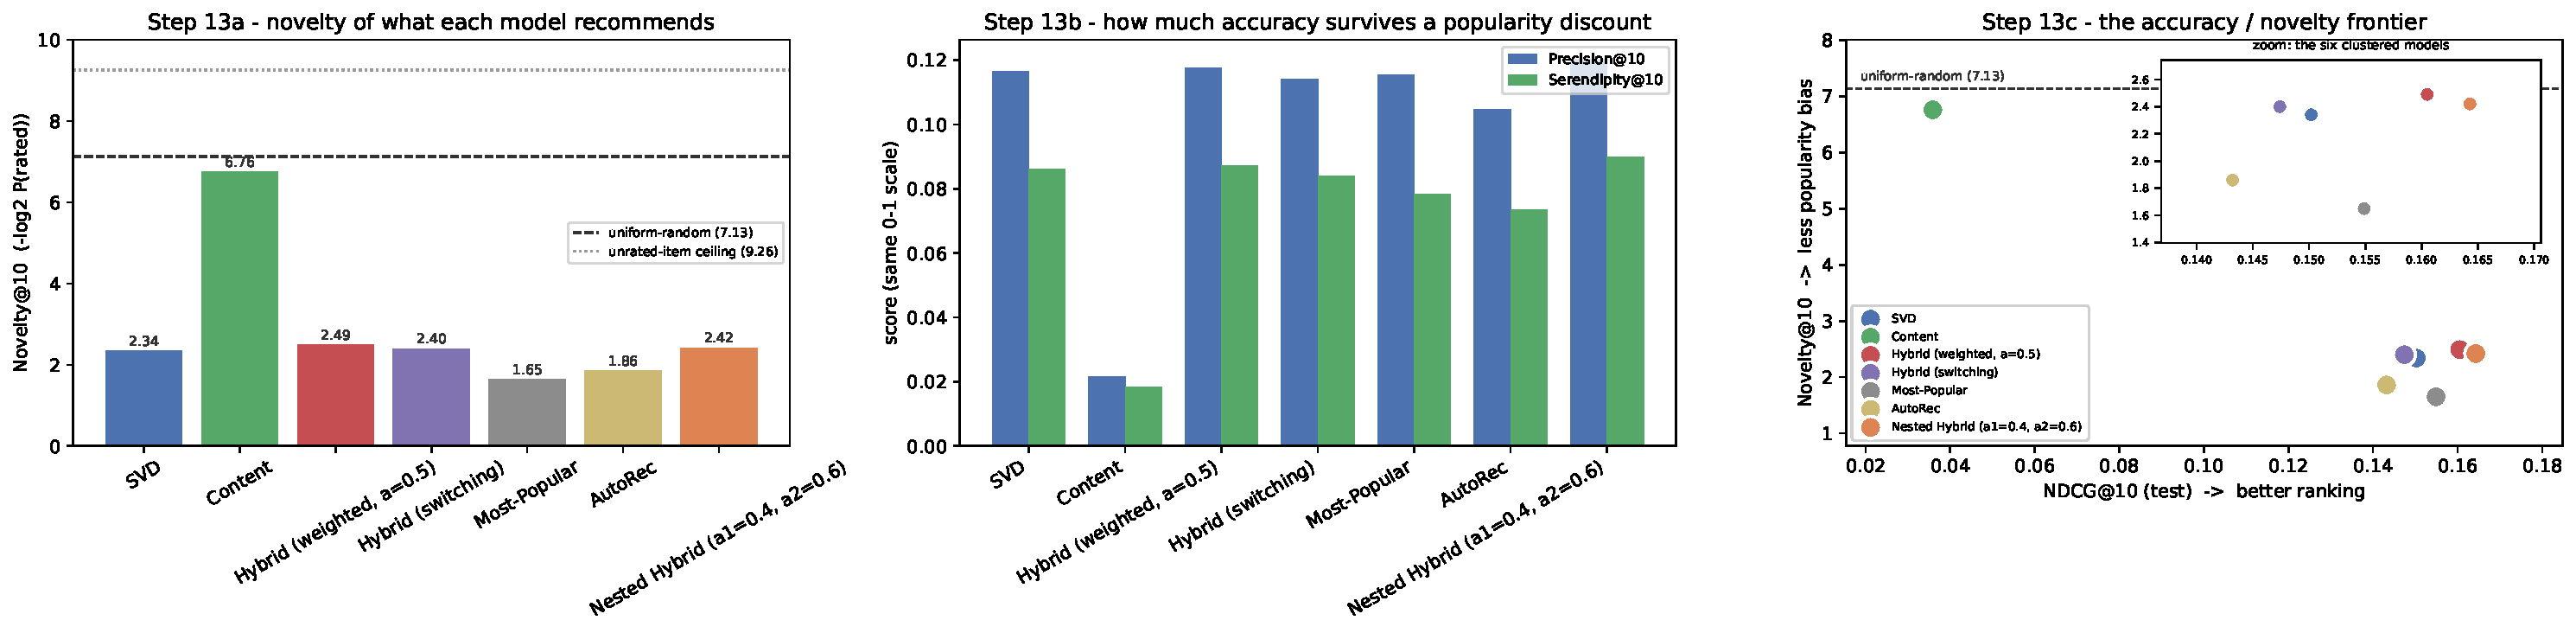
\includegraphics[width=0.98\textwidth]{fig3_beyond.pdf}
\caption{Beyond-accuracy results. Left: novelty of what each model
recommends, against the uniform-random line (7.13) and the unrated-item
ceiling (9.26). Centre: serendipity beside precision on the same scale.
Right: the accuracy/novelty frontier --- if any model dominated it would sit
alone in the upper right, and none does. The inset zooms the six systems that
cluster below the random line.}
\label{fig:beyond}
\end{figure*}

\subsection{Cold start is a data problem}\label{sec:cold}
The 732 cold items provide a direct test of whether model capacity can
compensate for missing signal. For the SVD, the largest absolute difference
between the predicted rating on a cold item and the user's own mean is
$0.00\mathrm{e}{+}00$ across every such row, and RMSE on those rows equals the
user-mean baseline's exactly, at 0.9805. For I-AutoRec, the standard deviation
of a given user's predictions across all 732 cold items is
$0.00\mathrm{e}{+}00$, against 0.17 to 0.50 on a sample of 200 warm items for
the same users.

A deeper, non-linear model therefore does not solve cold start by being more
expressive. Both models are looking at an all-zero input and can only return a
constant. This is a mathematical consequence of the architectures rather than
a statistical finding, and Section~\ref{sec:robust} confirms it holds
unchanged on every split tested.

Content signal is what breaks the tie. The content model places 481 cold items
into top-10 lists out of 6,100 slots; the switching hybrid, which hands cold
items to the content component instead of averaging them against a flat
collaborative score, reaches 60; the weighted hybrid reaches 6; SVD, I-AutoRec
and Most-Popular reach none. The cap is the blend weight rather than the text:
Appendix~\ref{app:tmdb} reports that raising text coverage of cold items from
18\% to 98\% left the weighted hybrid's cold reach at exactly 6.

\subsection{Ablations}\label{sec:ablation}
Four ablations were run; Appendix~\ref{app:grids} gives the grids.

\begin{itemize}\itemsep2pt
\item \textbf{Item-bias term.} Removing it costs 0.0419 RMSE
      (Table~\ref{tab:rmse}).
\item \textbf{Genre tokens.} Adding genre tokens to the TF-IDF features hurt
      validation ranking quality and was rejected.
\item \textbf{Blend weight and fallback.} $\alpha = 0.5$ with the neutral
      fallback was selected on validation NDCG@10.
\item \textbf{Capacity and regularisation.} Validation RMSE improved
      monotonically with hidden width up to 200, while validation NDCG@10 was
      maximised at width 25 with the strongest weight decay tested --- the
      configuration whose validation RMSE, 1.0819, is worse than the user-mean
      baseline's. The two metric families select opposite ends of the same
      grid, which is the clearest single piece of evidence for this paper's
      thesis.
\end{itemize}

\subsection{Robustness across splits}\label{sec:robust}
\begin{table}[t]\centering\small
\begin{tabular}{lccc}
\toprule
Ordering & $|$diff$|$ & std & Holds \\
\midrule
Nested $>$ Hybrid (wtd)   & 0.0035 & 0.0008 & 4/4 \\
Hybrid (wtd) $>$ SVD      & 0.0103 & 0.0022 & 4/4 \\
Nested $>$ Most-Popular   & 0.0150 & 0.0076 & 4/4 \\
Most-Popular $>$ AutoRec  & 0.0073 & 0.0050 & 4/4 \\
SVD $>$ Hybrid (switch)   & 0.0025 & 0.0006 & 4/4 \\
SVD vs.\ Most-Popular     & 0.0012 & 0.0060 & \textbf{sign flips} \\
\bottomrule
\end{tabular}
\caption{Head-to-head NDCG@10 orderings, differenced within each of four
splits. Five of six hold on every split; the sixth does not.}
\label{tab:robust}
\end{table}

Every number above comes from one split. Following Meng et al. (2020), the
entire seven-model comparison was repeated on four splits --- the reported
seed plus three chosen in advance --- with hyperparameters held at the values
the reported split's validation set selected. Any single model's NDCG@10 moves
by up to 0.0123 between splits, so two models closer together than that on one
split cannot be called separable from that split alone.

Comparing pairwise within each split is the sharper test, because all seven
systems share the split and a generous split lifts them together; differencing
cancels that shared movement. Table~\ref{tab:robust} reports the result; every standard deviation in this paper is the sample standard deviation ($n-1$).

Eight of ten claims tested hold on all four splits. The exception is the SVD
comparison from Section~\ref{sec:ranking}. On the reported split SVD loses to
Most-Popular at all three cutoffs, but across four splits the difference
averages $+0.0012$ NDCG@10 and changes sign twice. The defensible claim is
therefore not that collaborative filtering is worse than recommending
best-sellers but that it cannot be distinguished from it --- which motivates
the hybrid just as strongly, and is a claim the evidence actually supports.

The hybrid's own advantage is unaffected: the weighted hybrids beat plain SVD
on every split by $+0.0103 \pm 0.0022$. The beyond-accuracy findings are
considerably more stable than the ranking ones --- the content model's
coverage is $24.9\% \pm 0.2\%$ and its novelty $6.74 \pm 0.03$ across all four
splits --- and the zero-variance cold-item result holds exactly, as the
argument in Section~\ref{sec:cold} requires.

\subsection{Error analysis}
Three failures are worth reporting. First, selection noise is visible at this
scale: the nested hybrid's validation grid was won by a degenerate corner,
$\alpha_1 = 0$ and $\alpha_2 = 1$, which reduces the three-model system to
I-AutoRec alone. It beat the best genuine three-model blend by 0.0006 NDCG@10
on validation and then lost to it on test by 0.0211, 0.1432 against 0.1643.
Differences in the fourth decimal on a validation set of roughly 600 users
should not be treated as real, and the reported system uses the interior blend
for that reason.

Second, expanding the plot-text corpus improved the content model's coverage
and made its ranking worse. Cold items are 2.92\% of the relevant held-out
ratings, so promoting one into a top-10 usually costs a slot a popular item
would have converted. Offline ranking metrics can credit only items somebody
already rated and therefore penalise discovery systematically; this is a
limitation of the evaluation, not a regression in the model.

Third, the switching hybrid ranks consistently below plain SVD, by
$0.0025 \pm 0.0006$ across four splits, while reaching 60 cold-start slots
against SVD's zero. That single pair contains the accuracy/coverage trade-off
in both directions, and both directions are separable.

%%%%%%%%%%%%%%%%%%%%%%%%%%%%%%%%%%%%%%%%%%%%%%%%%%%%%%%%%%%%%%%%%%%%%%%%%%%
\section{Conclusion}

Seven movie recommenders were built and evaluated on one held-out split under
five families of measure. The nested hybrid ranks best (NDCG@10 0.1643) and is
the most serendipitous; I-AutoRec has the lowest rating error (0.8517) while
recommending from 0.6\% of the catalogue, the same fraction as a
non-personalized baseline and from the same end of the popularity
distribution; the content model is the most diverse and the worst ranker.
Three different models hold the six available titles, so reporting a single
best model would have concealed the result rather than summarising it.

Composability mattered as much as any individual model. Because a hybrid can
take another hybrid as a component, the three-model system is two lines of
composition, and because the components remain separately measurable, the
attribution in Section~\ref{sec:beyond} is possible at all.

The main limitations are: one dataset and one domain, so conclusions about
capacity are tied to this scale; offline evaluation only, which penalises
discovery by construction; hyperparameters selected on one validation split,
so Section~\ref{sec:robust} measures split variance rather than selection
variance; and a serving layer that scores a fixed set of users in advance, so
a new user receives the popularity baseline until the next batch run.

Three extensions follow directly. An online or interleaved evaluation would
test whether the coverage the content model buys is worth the offline ranking
it costs. Repeated splits for hyperparameter \emph{selection}, not only for
reporting, would capture selection variance. And feeding content features into
the deep model rather than blending them afterwards --- a two-tower design, or
injecting text similarities into the hidden layer --- would address the fact
that all 732 cold items have plot text I-AutoRec cannot see. That trade-off
runs both ways: late fusion is what keeps each component separately
measurable, and it is what allowed this project to show that I-AutoRec
collapses onto popularity while the content model does not.

%%%%%%%%%%%%%%%%%%%%%%%%%%%%%%%%%%%%%%%%%%%%%%%%%%%%%%%%%%%%%%%%%%%%%%%%%%%
\begin{apareferences}

Adomavicius, G., \& Kwon, Y. (2012). Improving aggregate recommendation
diversity using ranking-based techniques. \textit{IEEE Transactions on
Knowledge and Data Engineering, 24}(5), 896--911.
\url{https://doi.org/10.1109/TKDE.2011.15}

Burke, R. (2002). Hybrid recommender systems: Survey and experiments.
\textit{User Modeling and User-Adapted Interaction, 12}(4), 331--370.
\url{https://doi.org/10.1023/A:1021240730564}

Cremonesi, P., Koren, Y., \& Turrin, R. (2010). Performance of recommender
algorithms on top-N recommendation tasks. In \textit{Proceedings of the Fourth
ACM Conference on Recommender Systems} (pp. 39--46). Association for Computing
Machinery. \url{https://doi.org/10.1145/1864708.1864721}

Harper, F. M., \& Konstan, J. A. (2015). The MovieLens datasets: History and
context. \textit{ACM Transactions on Interactive Intelligent Systems, 5}(4),
Article 19. \url{https://doi.org/10.1145/2827872}

He, X., Liao, L., Zhang, H., Nie, L., Hu, X., \& Chua, T.-S. (2017). Neural
collaborative filtering. In \textit{Proceedings of the 26th International
Conference on World Wide Web} (pp. 173--182). International World Wide Web
Conferences Steering Committee. \url{https://doi.org/10.1145/3038912.3052569}

Kaminskas, M., \& Bridge, D. (2016). Diversity, serendipity, novelty, and
coverage: A survey and empirical analysis of beyond-accuracy objectives in
recommender systems. \textit{ACM Transactions on Interactive Intelligent
Systems, 7}(1), Article 2. \url{https://doi.org/10.1145/2926720}

Koren, Y., Bell, R., \& Volinsky, C. (2009). Matrix factorization techniques
for recommender systems. \textit{Computer, 42}(8), 30--37.
\url{https://doi.org/10.1109/MC.2009.263}

Meng, Z., McCreadie, R., Macdonald, C., \& Ounis, I. (2020). Exploring data
splitting strategies for the evaluation of recommendation models. In
\textit{Proceedings of the 14th ACM Conference on Recommender Systems}
(pp. 681--686). Association for Computing Machinery.
\url{https://doi.org/10.1145/3383313.3418479}

Panda, D. K., \& Ray, S. (2022). Approaches and algorithms to mitigate cold
start problems in recommender systems: A systematic literature review.
\textit{Journal of Intelligent Information Systems, 59}(2), 341--366.
\url{https://doi.org/10.1007/s10844-022-00698-5}

Sarwar, B., Karypis, G., Konstan, J., \& Riedl, J. (2001). Item-based
collaborative filtering recommendation algorithms. In \textit{Proceedings of
the 10th International Conference on World Wide Web} (pp. 285--295).
Association for Computing Machinery.
\url{https://doi.org/10.1145/371920.372071}

Sedhain, S., Menon, A. K., Sanner, S., \& Xie, L. (2015). AutoRec:
Autoencoders meet collaborative filtering. In \textit{Proceedings of the 24th
International Conference on World Wide Web} (pp. 111--112). Association for
Computing Machinery. \url{https://doi.org/10.1145/2740908.2742726}

\end{apareferences}

%%%%%%%%%%%%%%%%%%%%%%%%%%%%%%%%%%%%%%%%%%%%%%%%%%%%%%%%%%%%%%%%%%%%%%%%%%%
\appendix
\section{Expanding plot-text coverage}\label{app:tmdb}
The TMDB corpus originally covered 3,536 of the 9,724 rated films (36.4\%),
and only 18\% of cold items. It was expanded to 9,603 films (98.8\%) and 98\%
of cold items. The effect on the content model was measured rather than
assumed: cold-start reach roughly tripled, from 163 to 481 top-10 slots, and
catalogue coverage rose from 17.8\% to 24.9\%, while ranking quality fell,
NDCG@10 going from 0.0469 to 0.0359.

An earlier version of this project predicted that the weighted hybrid's
cold-start reach was capped by text coverage. That prediction was tested and
is wrong: coverage of cold items went from 18\% to 98\% and the weighted
hybrid's reach stayed at exactly 6 slots out of 6,100. The real cap is the
blend weight. A cold item has no collaborative signal, so its standardised
collaborative score sits at the user's own mean, and at $\alpha = 0.5$ the
content half cannot lift it past warm items scoring well on both halves. The
switching hybrid, which does not average against a flat score, is the variant
whose reach improved, from 38 to 60 slots.

\section{Hyperparameter grids}\label{app:grids}
\begin{table}[h]\centering\small
\begin{tabular}{llccc}
\toprule
$h$ & decay & val RMSE & val NDCG@10 & epoch \\
\midrule
25  & $10^{-5}$ & 0.9035 & 0.0382 & 205 \\
25  & $10^{-4}$ & 0.9004 & 0.0436 & 196 \\
25  & $10^{-3}$ & 0.8891 & 0.0830 & 374 \\
25  & $10^{-2}$ & 1.0819 & \textbf{0.1196} & 413 \\
200 & $10^{-5}$ & 0.8629 & 0.0656 & 67 \\
200 & $10^{-4}$ & \textbf{0.8616} & 0.0721 & 67 \\
200 & $10^{-3}$ & 0.8634 & 0.0853 & 75 \\
200 & $10^{-2}$ & 0.9093 & 0.0942 & 2831 \\
\bottomrule
\end{tabular}
\caption{I-AutoRec validation grid. The two metric families select opposite
ends of it.}
\label{tab:autogrid}
\end{table}

\TODO{Add the SVD $k \times$ damping grid and the $\alpha$ sweep table here
from notebook Steps 2 and 7. Both already print as tables in the notebook.}

\section{Robustness across splits}\label{app:seeds}
\begin{table}[h]\centering\footnotesize
\begin{tabular}{lccccc}
\toprule
Model & s1 & s42 & s12345 & reported & std \\
\midrule
SVD                & 0.1529 & 0.1545 & 0.1585 & 0.1502 & 0.0035 \\
Content            & 0.0341 & 0.0351 & 0.0352 & 0.0359 & 0.0007 \\
Hybrid (weighted)  & 0.1601 & 0.1664 & 0.1703 & 0.1605 & 0.0049 \\
Hybrid (switching) & 0.1504 & 0.1527 & 0.1553 & 0.1474 & 0.0034 \\
Most-Popular       & 0.1560 & 0.1468 & 0.1536 & 0.1549 & 0.0041 \\
I-AutoRec          & 0.1453 & 0.1407 & 0.1530 & 0.1432 & 0.0053 \\
Nested Hybrid      & 0.1638 & 0.1705 & 0.1726 & 0.1643 & 0.0044 \\
\bottomrule
\end{tabular}
\caption{NDCG@10 across four splits. Widest swing for any single model:
0.0123.}
\label{tab:seeds}
\end{table}

Coverage and novelty are markedly more stable than ranking. Across the same
four splits, coverage is $24.9\% \pm 0.2\%$ for the content model,
$5.5\% \pm 0.0\%$ for the weighted hybrid and $0.6\% \pm 0.0\%$ for both
I-AutoRec and Most-Popular; novelty is $6.74 \pm 0.03$, $2.50 \pm 0.02$,
$1.84 \pm 0.07$ and $1.64 \pm 0.01$ respectively. Rating error is
$0.8466 \pm 0.0061$ for I-AutoRec and $0.8664 \pm 0.0077$ for the SVD.

\textit{Caveat.} Hyperparameters were selected on the reported split's
validation set and held fixed, so some of that data lands in another split's
test set. The optimism this introduces is small, because the choices are
coarse, but it is real: this measures split variance with the model fixed, not
selection variance.

\section{Deployment}\label{app:deploy}
\begin{figure}[h]
\centering
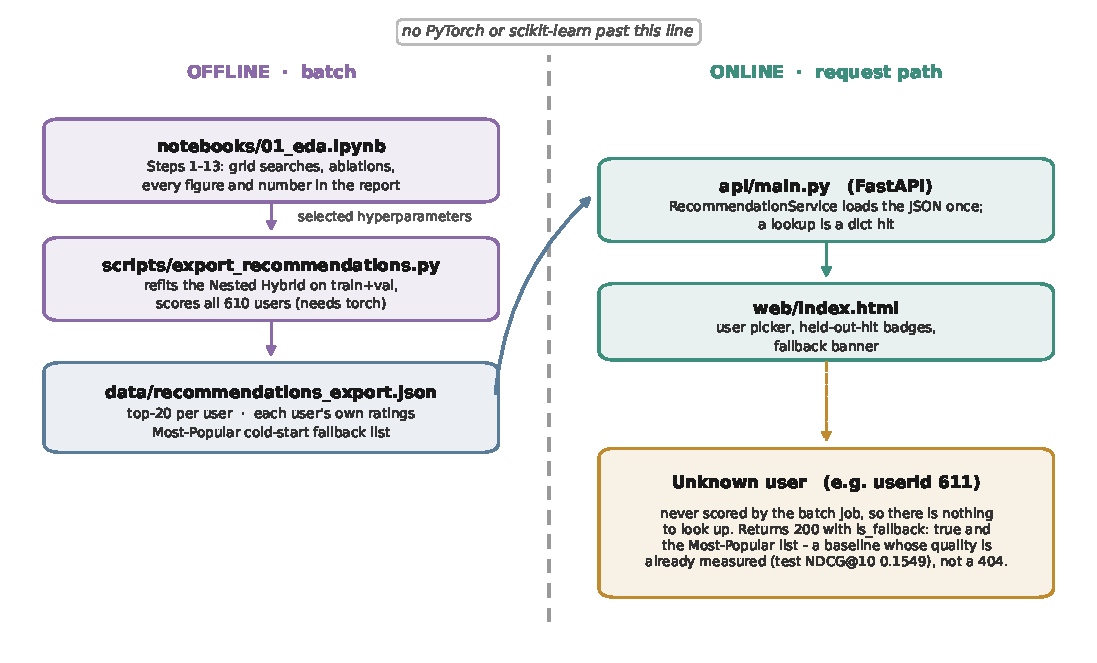
\includegraphics[width=\columnwidth]{fig2_serving.pdf}
\caption{Batch/serving split. The batch job fits and scores; the serving tier
reads the resulting table. No training framework is loaded in the request
path.}
\label{fig:serving}
\end{figure}

A batch script refits the deployed nested hybrid on train${+}$validation,
scores all 610 users and writes a JSON lookup table. The serving process reads
that file and never imports PyTorch or scikit-learn, so a recommendation is a
dictionary lookup. A user the batch job never scored is answered with the
Most-Popular list and an explicit flag rather than an error; because that
fallback is the same baseline evaluated in Table~\ref{tab:ndcg}, its quality is
a reported number rather than a guess.

Across all 610 users, 192 recommendations in the top ten are films the user
really did rate --- in the test split, which the model was never fitted on.
166 of the 610 users see at least one. These are held-out hits rather than
leakage, and the interface labels them as such.

\section{Declarations}\label{app:decl}
\noindent\textbf{Individual contribution.} This project was completed
individually. All code, experiments, figures and writing are the author's own
work.

\TODO{The brief links the AUT Academic Integrity policy but does not mandate
an AI-use declaration table. Including one costs nothing and protects you.
Add it here, or delete this note if you decide against it.}

\end{document}
